\documentclass[a4paper, 11pt]{article}
\usepackage{comment} % enables the use of multi-line comments (\ifx \fi) 
\usepackage{fullpage} % changes the margin
\usepackage{amsmath}
\usepackage[makeroom]{cancel}

\usepackage{graphicx}
\usepackage[]{textcomp}
\usepackage{subcaption}

\usepackage{tikz}
\usetikzlibrary{arrows,automata}
\usepackage{fixltx2e}
\newcommand\tab[1][1cm]{\hspace*{#1}}

\usepackage{geometry}
 \geometry{
 a4paper,
 left=15mm,
 right=15mm,
 top=15mm,
 }

\begin{document}
\noindent \includegraphics[scale=0.2]{figures/logo.png}\\
\large \textbf{Systèmes Logiques - EE102}\hfill \textbf{Valentin RIAT - SCIPER: 289121}\\
 \hfill \large \textbf{Projet de semestre: Réveil-matin de voyage}\hfill \textbf{Rafael RIBER - SCIPER: 296142}\\
 \large \textbf{EL-BA2 - 2018-2019} \hfill \large \textbf{Groupe 6}

\section{Déscription générale et mode d'emploi}
Notre projet consiste en un réveil-matin de voyage avec fonctions annexes, réalisé sur la carte de développement DE10-Lite. Deux boutons permettent de passer d'un mode de fonctionnement à l'autre. Un bouton rotatif permet l'interfaçage avec les modes, et un interrupteur permet d'activer ou désactiver le réveil.
\subsection{Mode d'emploi}
\begin{minipage}{0.6\textwidth}
\begin{itemize}
\item Dans n'importe quel mode:
\begin{itemize}
\item Changer de mode: Presser B1 ou B2
\item Activer/Désactiver le réveil: \\Interrupteur "Réveil ON/OFF" (une LED indique si le réveil est activé)
\item Désactiver le buzzer en cas d'alarme: Appuyer sur le bouton rotatif
\end{itemize}
\item Mode 1: Affichage de l'heure
\item Mode 2: Réglage de l'heure:\\
Tourner le bouton rotatif pour choisir la valeur sélectionnée (qui clignote). Et presser le bouton rotatif pour passer à la valeur suivante. Une fois l'heure choisie entrée, un retour à un autre mode règle l'heure.
\item Mode 3: Réglage du réveil.\\Le réglage s'effectue comme le mode 2.
\item Mode 4: Chronomètre\\
Une pression sur le bouton rotatif démarre ou arrête le chronomètre. Une longue pression le remet à zéro.
\item Mode 5: Choix du ton de l'alarme.\\ Tourner le bouton rotatif jusqu'à la valeur désirée (0 à 15). Une valeur plus haute signifie un ton plus grave. Une fois la valeur choisie, changer de mode règle le ton de l'alarme.
\item Mode 6: Mode Fun :)
\item Mode 7: Mode Nuit: Désactive l'affichage pour un sommeil tranquille
\end{itemize}
\end{minipage}
\begin{minipage}{0.4\textwidth}
\includegraphics[scale=0.4]{figures/de10label.png}
\end{minipage}
\newpage
\section{Solutions techniques}
\subsection{Machine d'états finis générale}
\begin{center}
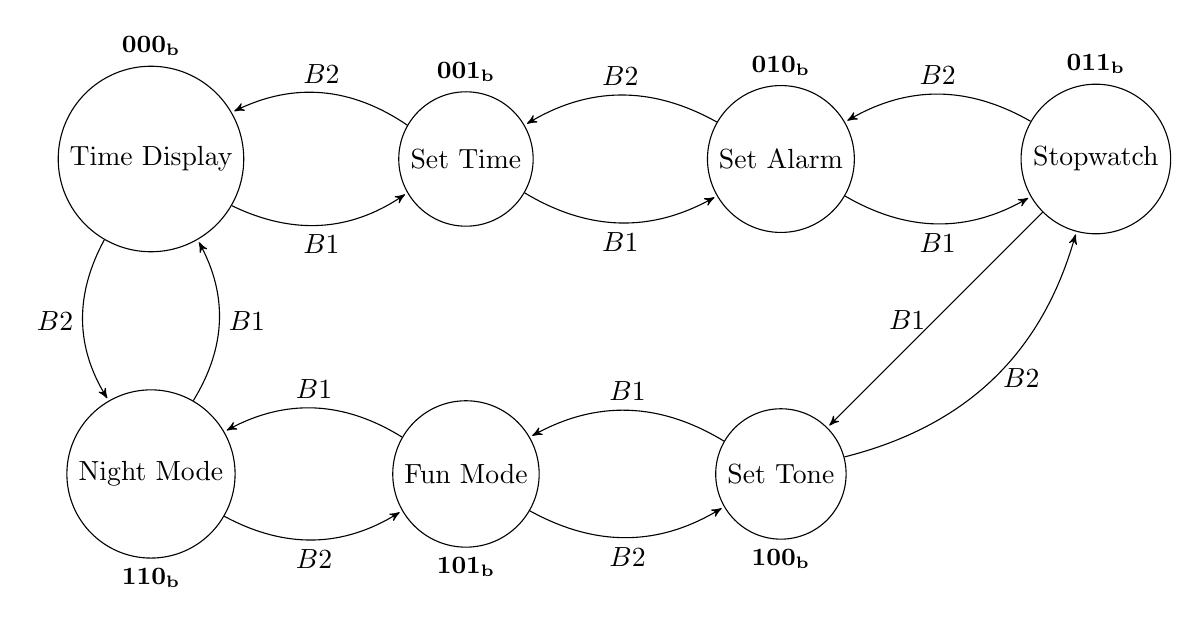
\begin{tikzpicture}[->,>=stealth',shorten >=1pt,auto,node distance=4cm,
        scale = 1,transform shape]

  \node[state][label={\small\textbf{000\textsubscript{b}}}] (Time Display) [] {Time Display};
  
  \node[state][label={\small\textbf{001\textsubscript{b}}}] (Set Time) [right of=Time Display] {Set Time};
  
  \node[state][label={\small\textbf{010\textsubscript{b}}}] (Set Alarm) [right of=Set Time] {Set Alarm};
  \node[state][label={\small\textbf{011\textsubscript{b}}}] (Chronometer) [right of=Set Alarm] {Stopwatch};
  \node[state][label=below:{\small\textbf{100\textsubscript{b}}}] (Set Tone) [below of=Set Alarm] {Set Tone};
  \node[state][label=below:{\small\textbf{101\textsubscript{b}}}] (Fun Mode) [left of=Set Tone] {Fun Mode};
  \node[state][label=below:{\small\textbf{110\textsubscript{b}}}] (Night Mode) [below of=Time Display] {Night Mode};

  \path (Time Display) edge [bend right]           node[below] {$B1$} (Set Time)
  		(Set Time) edge [bend right]           node[below] {$B1$} (Set Alarm)
        (Set Alarm) edge [bend right]              node[below] {$B1$} (Chronometer)
        (Chronometer) edge				node[left] {$B1$} (Set Tone)
        
       
        (Set Tone) edge [bend right]            node[above] {$B1$} (Fun Mode)
        (Fun Mode) edge  [bend right]             node[above] {$B1$} (Night Mode)
        (Night Mode) edge [bend right]               node[right] {$B1$} (Time Display)
        
        
  		(Time Display) edge[bend right]              node[left] {$B2$} (Night Mode)
        (Night Mode) edge[bend right]              node[below] {$B2$} (Fun Mode)
        (Fun Mode) edge[bend right]              node[below] {$B2$} (Set Tone)
        (Set Tone) edge	[bend right]			node[right] {$B2$} (Chronometer)
        
        (Chronometer) edge[bend right]              node[above] {$B2$} (Set Alarm)
        (Set Alarm) edge[bend right]              node [above]{$B2$} (Set Time)
        (Set Time) edge[bend right]              node [above]{$B2$} (Time Display);
\end{tikzpicture}
\end{center}
\subsection{Machines d'états finis secondaires et solutions techniques}
\subsubsection{Détection de flancs}
Les circuits les plus utiles que nous avons développés sont des détecteurs de flancs montants (Fig. \ref{fig:risingEdge}) et déscendants (Fig. \ref{fig:fallingEdge}) ces circuits sont notament utilisés lors du décodage du bouton rotatif.



\begin{figure}[h]
\centering
\begin{subfigure}{.5\textwidth}
  \centering
  \includegraphics[width=.7\linewidth]{figures/risingEdge.png}
  \caption{Détection de flanc montant}
  \label{fig:risingEdge}
\end{subfigure}%
\begin{subfigure}{.5\textwidth}
  \centering
  \includegraphics[width=.7\linewidth]{figures/fallingEdge.png}
  \caption{Détection de flanc déscendant}
  \label{fig:fallingEdge}
\end{subfigure}
\caption{Circuits de détection de flancs}
\label{fig:edge}
\end{figure}

\subsubsection{Debounce}
Nous utilisons une série de D-Latch (Fig. \ref{fig:debounce}) en cascade afin de debounce les boutons.

\begin{figure}[!h]
\centering
\includegraphics[scale=0.4]{figures/debounce.png}
\caption{Circuit de debounce}
\label{fig:debounce}
\end{figure}
\newpage
\subsubsection{Décodage du bouton rotatif}
Les trois canaux (CHA, CHB, CHC) du bouton rotatif passent tout d'abord par un circuit de debounce Ensuite, un décodeur (decod\_rotation\_logic) prend les valeurs courantes et précédentes et active la sortie \textbf{EN} si une rotation est effectuée, ainsi que la sortie correspondante au sens de rotation (\textbf{C}lock\textbf{W}ise ou \textbf{C}ounter\textbf{C}lock\textbf{W}ise). Afin de palier à une double activation de EN, nous utilisons un compteur comptant jusqu'à un. Toutes les sorties passent ensuite par un détecteur de flanc montant, qui active la sortie durant un cycle d'horloge.

\begin{figure}[h]
\centering
\includegraphics[scale=0.5]{figures/decodeRot.png}
\caption{Décodeur du bouton rotatif}
\label{fig:decodeRot}
\end{figure}
\subsubsection{FSM d'affichage de texte}
Une machine d'états finis (Fig. \ref{fig:textFSM}) nous permet d'afficher un texte lors de l'arrivée sur le mode d'affichage de texte. Un compteur est dimensionné pour afficher un texte durant 0.5 secondes.
\begin{figure}[h]
\centering
\includegraphics[scale=0.4]{figures/TextFSM.png}
\caption{FSM d'affichage de texte sur un intervalle de temps}
\label{fig:textFSM}
\end{figure}


\end{document}